\chapter{Ondes Stationnaires}
\section{Introduction}
\begin{marginfigure}[3cm]
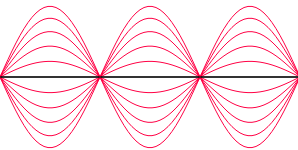
\includegraphics[width=5cm]{7_1.png}
\caption{Chaque trait indique un temps différent. Nous pouvons observer les noeuds et les ventres caractéristiques des ondes stationnaires, ainsi que la séparation des variables. }
\label{7_1}
\end{marginfigure}
%Nous avons étudié jusqu'à présent la propagation d'une seule onde et les phénomènes de réflexion sur celle-ci. 
Dans ce chapitre nous allons observer des phénomènes d'interférence d'ondes qui se propagent dans des environnement restreints.
A l'intérieur de cet environnement, des réflexions multiples peuvent apparaître. Ces réflexions diverses créeront ce que l'on appelle des ondes stationnaires si certaines conditions sont respectées.
En effet, si les ondes réfléchies sont toutes en phase, une interférence constructive se produit. Ce type d'onde stationnaire ne se produit que pour des fréquences particulières que nous allons déterminer dans les sections suivantes, et qui dépendent de la taille de l'environnement restreint considéré.
\begin{marginfigure}
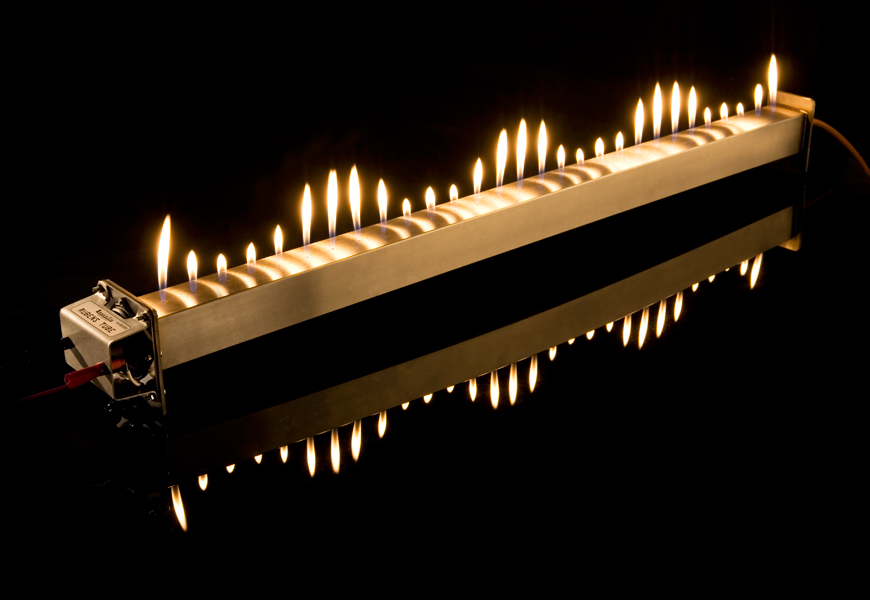
\includegraphics[width=\linewidth]{rubenstube}
\caption{Le \textit{tube de Rubens} est un outil pour visualiser des ondes stationnaires acoustiques. Il s'agit d'un tube perforé dans lequel on introduit du gaz d'un côté et on place un haut-parleur de l'autre. La hauteur des flammes est proportionnel à la pression, c'est donc aux ventres de pression que l'on retrouve les plus hautes flammes.  }
\end{marginfigure}
\par Comme l'illustre l'exemple ci-dessous, nous pouvons reconnaître une onde stationnaire d'un point de vue mathématique car elle peut être décomposée en un produit de deux fonctions, une dépendante du temps et l'autre de la position(visible sur la figure de droite). C'est la raison pour laquelle nous allons utiliser la technique des variables séparables pour résoudre les problèmes facilement. Une autre possibilité de résolution serait de calculer les champs réfléchis une multitude de fois sur les interfaces et sommer les résultats. Il s'agit là d'une vue physique du problème, mais est impraticable du point de vue mathématique.
\par Le terme "onde stationnaire" provient de l'observation visuelle que l'on peut faire du phénomène, par exemple dans le cas d'une corde vibrante. Lorsque nous avons affaire à une onde stationnaire à une fréquence fixée, nous n'observons plus le déplacement de l'onde. On observe alors des points de la corde qui ne bougent pas, et d'autres où le déplacement vertical est maximal. Les points qui ne bougent pas sont appelées les nœuds et les points à déplacement maximal sont les ventres. De plus, la forme générale de la corde suit une sinusoïde, dont les crêtes correspondent toujours aux ventres et les zéros correspondent toujours aux nœuds. Il est donc logique de dire que, pour une onde stationnaire à une fréquence fixée, un nœud (ventre) se trouve toujours à une distance égale de deux ventres (nœuds).
%Les principales caractéristiques des ondes stationnaires sont que l'équation qui la représente peut être décomposée le déplacement de l'onde n'est 
\section{Illustration du phénomène}
Dans cette section, en guise d'illustration, nous allons développer l'interférence créée par deux ondes se propageant dans des sens contraires. Définissons deux ondes électromagnétiques transverses A et B, de pulsations respectives $\omega_a$ et $\omega_b$ et polarisées linéairement selon l'axe z. Supposons qu'elles se propagent dans la direction $+x$ et $-x$ respectivement, et ne dépendent toutes les deux que de leur coordonnée\footnote{Il peut s'agir par exemple d'une onde se propageant sur une corde ou un tube positionné le long de l'axe des $x$, ou encore d'une onde plane se propageant dans la direction de l'axe des $x$.} en $x$. Les deux ondes peuvent s'écrire comme 
$$ \vec{E_a}=A_a\cos(\omega_a t+ \phi_a-k_ax) \hat{e_z}$$
$$ \vec{E_b}=A_b\cos(\omega_b t+\phi_b+k_bx) \hat{e_z},$$
où $\phi_a$ et $\phi_b$ dénotent le déphasage des ondes A et B respectivement, et où $k_a$ et $k_b$ sont leurs nombres d'onde.
Nous allons calculer l'onde résultante de la somme de ces deux ondes: 
$$ \vec{E}=A_a\cos(\omega_a t+\phi_a-k_ax) \hat{e_z} + A_b\cos(\omega_b t+\phi_b+k_bx) \hat{e_z}.$$
L'onde stationnaire peut se produire uniquement sur l'axe x et nous pouvons nous concentrer sur la composante selon $z$ uniquement, les autres étant nulles:
$$ E_z=A_a\cos(\omega_a t+\phi_a-k_ax) + A_b\cos(\omega_b t+\phi_b+k_bx).$$
Une des premières conditions à imposer est que les amplitudes des deux ondes soient égales ($A_a=A_b=A$). Dans ce cas, nous pouvons transformer la somme des deux cosinus en un produit: 
\begin{eqnarray}
E_z&=&2A\cos\left(\frac{\omega_a t+\phi_a-k_ax+\omega_b t+\phi_b+k_bx}{2}\right)\nonumber \\&.&\cos\left(\frac{\omega_a t+\phi_a-k_ax-\omega_b t-\phi_b-k_bx}{2}\right).
\end{eqnarray}
On observe directement que pour obtenir deux fonctions à variables "séparées", il nous faut imposer une autre condition : les fréquences doivent être identiques ($\omega_a=\omega_b=\omega)$. Dans ce cas, sachant que les ondes se propagent dans le même milieu, et donc à la même vitesse, on obtient que $k_a=k_b=k$. Au final, on observe que l'onde résultante peut s'écrire comme le produit de deux facteurs dont l'un dépend uniquement du temps et l'autre de la position:
$$ E_z=2A\cos(\omega t+\frac{\phi_a+\phi_b}{2})\cos(kx-\frac{\phi_a-\phi_b}{2}).$$

Les origines de ces ondes stationnaires sont multiples. D'une part nous pouvons avoir tout simplement deux ondes créées séparément qui se propagent dans des sens opposés mais ce phénomène est rare car les conditions pour qu'il y ait onde stationnaire sont difficiles à respecter. Le plus souvent, ce phénomène apparaîtra lorsque une onde se propage entre deux interfaces. Il peut alors se produire des réflexions multiples. L'onde incidente est réfléchie sur la première interface, créant l'onde qui se propage dans la direction opposée. Elle est ensuite  réfléchie sur la seconde et réfléchie à nouveau sur la première, etc. Les réflexions successives permettent d'"entretenir" les deux ondes dans les deux directions opposées, obtenant ainsi une onde stationnaire d'amplitude élevée. Ceci n'est néanmoins possible que si l'onde réfléchie par la deuxième interface vient s'additionner {\it en phase} avec l'onde initiale. Il y a donc des conditions sur les distances entre ces interfaces. Comme indiqué plus haut, l'analyse complète des réflexions successives est cependant ardue, et il est plus simple mathématiquement de simplement rechercher si la solution "à variables séparées" est possible pour la configuration considérée. C'est cette méthode que nous allons utiliser dans le reste du chapitre.


\section{Résolution par variables séparables}
Nous savons ici que la solution de notre équation d'onde sera une fonction à variables séparables donc nous allons utiliser cette technique pour résoudre le problème. Nous allons d'abord résoudre le problème pour une configuration à une dimension, et ensuite nous pourrons généraliser le problème en 2 et 3 dimensions.

Considérons un environnement avec deux interfaces en $x=0$ et $x=L$ entre lesquelles se propagent des ondes qui ne dépendent que de la coordonnée en $x$ (par exemple un tube, une corde, ou des ondes électromagnétiques planes entre 2 plaques métalliques). L'équation d'onde en 1D s'écrit 
\[ \frac{\partial^2\phi(x,t)}{\partial x^2} = \frac{1}{v^2}\frac{\partial^2\phi(x,t)}{\partial t^2}, \]
où $\phi(x,t)$ est l'onde stationnaire recherchée, et où $v$ est la vitesse de propagation des ondes dans le milieu considéré. Nous supposons que la solution à cette fonction est une solution de la forme $\phi(x,t)=X(x)T(t)$. Nous allons injecter cette solution dans l'équation d'onde. Pour alléger l'écriture, nous allons utiliser les notations $X'=\frac{dX}{dx}$, et $T'=\frac{dT}{dt}$. Celles-ci sont possibles car les fonctions X et T sont des fonctions à une seule variable. L'équation d'onde se réécrit comme
\[ \frac{\partial^2}{\partial x^2}(X(x)T(t)) = \frac{1}{v^2}\frac{\partial^2}{\partial t^2}(X(x)T(t)), \]
ce qui devient, avec la notation simplifiée, 
\[ X''T=\frac{1}{v^2}T''X\]
ou encore
\begin{equation}
\frac{X''}{X}=\frac{1}{v^2}\frac{T''}{T}=\mbox{constante}.
\label{eq:X''Cst}
\end{equation}
Dans (\ref{eq:X''Cst}), les deux membres ne dépendent respectivement que de $x$ et que de $t$. Puisqu'ils sont toujours égaux, ils ne peuvent qu'être constants. Nous définissons ensuite 3 cas. Cette constante vaut soit $k^2, 0$ ou$-k^2$ avec $k\in \mathbb{R}$.
Prenons le cas où la constante vaut $0$. Nous avons la solution triviale $X=0$, $T=0$ et par conséquent $\phi(x,t)=0$.
Ensuite, le cas où la constante vaut  $k^2$ nous mène à une solution de type
\[X(x)=A\exp(kx)+B\exp(-kx) \]
\[T(t)=C\exp(kvt)+D\exp(-kvt) \]
Nous allons voir dans les sections suivantes les conditions limites à imposer. Par exemple, pour une corde vibrante de longueur $L$, fixée aux deux extrémités, on a $X(0)=0$ et $X(L)=0$. Ces conditions limites imposent $C=0$ et $D=0$, dès lors, nous obtenons la même solution triviale $X(x)=0$ et donc $\phi(x,t)=0$. Pour obtenir des solutions oscillantes il nous faudra utiliser la constante $-k^2$. Dans ce cas, nous allons obtenir des solutions du type \sidenote{Nous verrons plus tard que la solution exacte comprend une somme infinie de $k$ et $\omega$ possibles.}

\[X(x)=A\exp(ikx)+B\exp(-ikx) = A'\sin(kx) + B' \cos(kx)\]
\[T(t)=C\exp(ikvt)+D\exp(-ikvt) = C'\sin(kvt) + D' cos(kvt) \]
\[\phi(x,t) = X(x) T(t)\]%  (A'\sin(kx) + B' \cos(kx))(C'\sin(kvt) + D' cos(kvt)). \]

Dans la section suivante, nous allons déterminer, avec les conditions limites adéquates, les valeurs de $k$. Par la suite, nous noterons $kv$ par $\omega=2\pi f$ qui est la pulsation.

\section{Conditions limites}
Nous avons établi la solution oscillante de l'équation d'onde, nous devons maintenant appliquer des conditions limites qui correspondent à la physique. Elles permettent de déterminer la valeur des constantes.
\subsection{Ondes mécaniques}
Pour la corde vibrante, il existe trois variables qui obéissent à l'équation d'onde, le déplacement vertical $y(x,t)$, la vitesse verticale $u(x,t)$ et la force verticale $F_y(x,t)$. La contrainte physique la plus fréquente est que la corde soit fixée à ses extrémités. Cela correspond à imposer un déplacement nul pour tout temps $t$ à ces deux positions, soit $y(0,t)=y(L,t)=0$. On résout donc l'équation d'onde en $y(x,t)$ en imposant ces deux conditions supplémentaires. 
\par Pour retrouver les autres valeurs, nous avons vu dans les chapitres précédents les équations couplées qui lient les différentes variables.On trouve la vitesse v en dérivant la position et la force avec une des équations constitutives.

\subsection{Ondes électromagnétiques}
De la même manière que pour la corde vibrante, il existe deux variables qui obéissent à l'équation d'onde dans le cas d'ondes électromagnétiques. Ces variables sont le champ électrique E et le champ magnétique H. Nous avons l'habitude de travailler avec le champ E plutôt que le champ H. Pour des interfaces qui sont composés de bons conducteurs, nous pouvons considérer ceux-ci comme des conducteurs parfaits. Dès lors, le champ électrique dans ce conducteur vaut zéro.
\subsection{Ondes acoustiques}
Plusieurs configurations sont possibles pour créer des ondes stationnaires acoustiques. Soit nous considérons l'extrémité d'un tube ouvert, soit fermé, les deux cas ne donneront pas lieu aux mêmes conditions limites. Les 3 variables obéissant à l'équation d'onde sont le déplacement\sidenote{En pratique, il y a bien entendu toujours une agitation thermique des molécules d'air qui vient s'ajouter aux déplacements que l'on considère ici, mais qui n'intervient pas dans le problème. En d'autres termes, le déplacement et la vitesse envisagés ici correspondent à des valeurs moyennées sur les déplacement liés à l'agitation thermique.} des particules d'air $\xi$, leur vitesse\sidenote{Il faut remarquer ici que cette vitesse est bien différente de la vitesse de l'onde et ne correspond pas non plus à la vitesse d'un éventuel flux d'air. L'air ambiant a bien une vitesse moyenne nulle et l'air ne "sort" pas du tube.} $u$ et la surpression par rapport à la pression atmosphérique $p$. 
\paragraph{Tube ouvert}
Dans ce cas, en tout temps, l'extrémité du tube est toujours à pression atmosphérique, par conséquent la surpression $p(x_e,t)=0$ à la position $x_e$ de l'extrémité considérée. 
\paragraph{Tube fermé}
Dans ce cas, il n'y a aucune particule d'air qui peut traverser la paroi. Dès lors, le déplacement ne peut être que nul en tout temps : $\xi(x_e,t)=0$.

\par Nous pouvons dès à présent mélanger les cas et étudier des tubes ouverts des deux côtés, fermés des deux côtés ou fermés d'un seul côté. Dans le dernier cas, appliquer les deux conditions limites sur la même variable ($\xi$, u ou p), ne sera pas directement possible. Il faut alors passer par les équations constitutives qui lient ces variables. Ces derniers font intervenir des dérivées, ce qui est la raison pour laquelle nous obtenons pour une pression minimale un déplacement maximal; un déplacement minimal, une pression maximale. 

\section{Modes propres}
Les conditions limites déterminent des valeurs possibles pour les coefficients $A', B', C', D'$ et le nombre d'onde $k$ (et $\omega$ par conséquent). La manière dont ces conditions aux limites sont définies déterminera aussi les fréquences auxquelles le système produira des ondes stationnaires.
Nous allons montrer deux exemples pour illustrer l'application des conditions limites. Dans les deux cas, notre condition initiale sera $\Phi(x,t=0)=0$. En premier, prenons par exemple une corde vibrante \sidenote{Cet exemple peut être adapté à beaucoup de cas, notamment avec les ondes acoustiques et électromagnétiques et les résultats seront identiques. Il faut néanmoins être prudent avant d'utiliser le résultat suivant et vérifier si les conditions limites sont compatibles.} avec les conditions limites $\xi(x=0)=\xi(x=L)=0$. Le fait d'imposer zéro en $x=0$ a pour conséquence de garder une fonction sinus et non cosinus pour la partie dépendante de la position. La condition initiale garde elle aussi la fonction sinus, c'est à dire $D'=0$. Ensuite, imposer un zéro en $x=L$ demande des valeurs de $k$ particulières: 
\[\xi(L,t)=A'C'\sin(kL)\sin(\omega t)=0\]
\[ kL = m\pi \leftrightarrow k=\frac{m\pi}{L},\] 
où $m$ est un entier positif. Les valeurs de $m$ sont les modes propres du système. Le premier mode possible, à savoir quand $m=1$, est appelé le mode fondamental. Tous les modes supérieurs à partir de $m=2$ sont appelés des harmoniques. Nous venons de montrer que seul certains nombres d'ondes sont des solutions de l'équation d'onde avec les conditions limites énoncées plus haut. Nous pouvons donc déterminer la liste des nombres d'ondes admis : 
$$ m = 1,2,3,4,5,...$$
$$ k = \frac{\pi}{L},\frac{2\pi}{L},\frac{3\pi}{L},\frac{4\pi}{L},\frac{5\pi}{L},...$$
$$ \lambda = 2L,\frac{2L}{3},\frac{2L}{4},\frac{2L}{5},\frac{2L}{6},... $$
La pulsation fondamentale est donnée par $\omega_1=\frac{\pi}{L}v$, la fréquence fondamentale est donc donnée par $f_1=\frac{v}{2L}$. Ensuite, on peut observer que, pour les conditions aux limites considérées ici, les fréquences des différents modes propres sont données par
$$ f_1,\; 2f_1,\; 3f_1,\; 4f_1,\; 5f_1,\; 6f_1, \ldots$$


\begin{figure}[h]\centering
	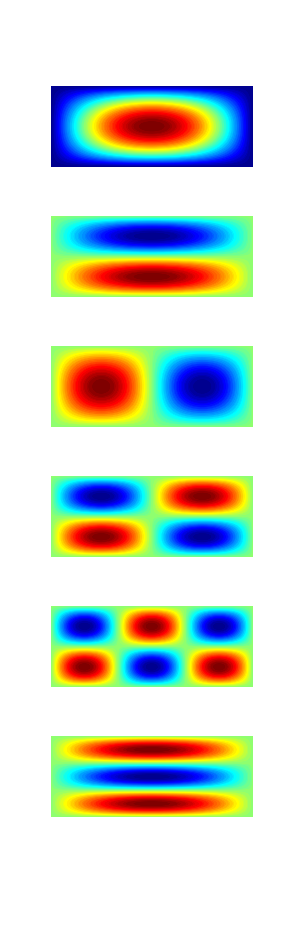
\includegraphics[width=10cm]{modes}
	\caption{Les 3 premiers modes propres}
\end{figure}

Deuxièmement, prenons le cas d'un tube ouvert d'un côté en $x=0$ et fermé en $x=L$. Nous allons appliquer les conditions limites suivantes, $p(0,t)=0$ et $\xi(L,t)=0$. Pour ce cas, nous choisissons de travailler avec la variable $p$. La condition limite en $x=0$ et la condition initiale impliquent donc
$$B' = D' = 0 \leftrightarrow p(x,t)=A''\sin(kx)\sin(\omega t)$$
Ensuite, le tube fermé implique un déplacement nul mais aussi une vitesse nulle. Grâce à l'équation constitutive $\frac{\partial p}{\partial x}=-\rho_0\frac{\partial u}{\partial t},$
on obtient
$$u(x,t)=A'''\cos(kx)\cos(\omega t)$$
$$\xi(x,t)=A''''\cos(kx)\sin(\omega t)$$
L'application de la condition aux limites est enfin possible, on a 
$$\xi(L,t)=0=A''''\cos(kL)\sin(\omega t) \leftrightarrow kL=m\pi + \pi/2$$
Le tableau obtenu précédemment se transforme de la façon suivante : 
$$ m = 1,2,3,4,5,6,...$$
$$ k = \frac{\pi}{2L},\frac{3\pi}{2L},\frac{5\pi}{2L},\frac{7\pi}{2L},\frac{9\pi}{2L},\frac{11\pi}{2L},...$$
$$ \lambda = 4L,\frac{4L}{3},\frac{4L}{5},\frac{4L}{7},\frac{4L}{9},\frac{4L}{11},... $$
Nous pouvons observer que ces résultats sont similaires mais pas identiques aux résultats précédents. C'est pour cela qu'appliquer machinalement les résultats du premier exemple est relativement dangereux. En particulier, la fréquence fondamentale vaut maintenant $f_1=\frac{v}{4L}$, et les fréquences propres sont données par
$$ f_1,\; 3f_1,\; 5f_1,\; 7f_1,\; 9f_1,\; 11f_1, \ldots$$

\section{Généralisation des modes propres}
Nous avons montré que plusieurs solutions peuvent exister pour une onde stationnaire qui correspondaient aux différents modes propres. Par le principe de superposition, il est aussi possible -- et c'est même ce qui arrive le plus fréquemment en pratique -- d'avoir un système qui oscille à plus que un mode propre.\sidenote{Rappelons la distinction entre les harmoniques et le timbre. Lorsqu'une note est jouée sur un instrument de musique, celle-ci aura un son différent du son créé par une harmonique de fréquence unique. En effet, le son de la guitare est composée d'une multitude d'harmoniques d'amplitude différentes. L'ensemble de ces harmoniques forment le timbre.} De manière générale, une infinité de mode propres est possible et donc la solution complète à l'équation d'onde devient une somme infinie comme suit : 
\[ \phi(x,t) = \sum_{m=1}^\infty(A_m'\sin(k_mx) + B_m' \cos(k_mx))(C_m'\sin(\omega_mt) + D' cos(\omega_mt)), \]
où les différentes constantes $A_m',B_m',C_m',D_m', k_m,\omega_m$ doivent satisfaire aux conditions aux limites pour chaque mode $m$.


\section{Généralisation en 3D}
Nous quittons un bref instant le monde 1D et allons tenter de généraliser les développements précédents en 3D. Pour cela nous avons besoin de l'équation d'onde générale. 
$$ \nabla^2 \phi = \frac{\partial^2\phi}{\partial\phi^2}$$
En coordonnées cartésiennes, elle s'écrit:
\begin{equation}
\frac{\partial^2\phi}{\partial x^2}+\frac{\partial^2\phi}{\partial y^2}+\frac{\partial^2\phi}{\partial z^2} = \frac{1}{v^2}\frac{\partial^2\phi}{\partial t^2}.
\label{eq:onde3D}
\end{equation}
La résolution se fait toujours par variables séparables mais il sera nécessaire de décomposer en plusieurs étapes. En premier lieu, on sépare la fonction du temps $T(t)$ telle que $\phi(x,y,z,t)=A(x,y,z)T(t)$. Ensuite on résout de nouveau $A(x,y,z)$ par variables séparables en répétant le processus jusqu'à obtenir 4 fonctions tels que $\phi(x,y,z,t)=X(x)Y(y)Z(z)T(t)$. Le raisonnement complet est réalisé dans le cours de Mathématiques 3, les résultats des fonctions $X$, $Y$, $Z$ seront tous des combinaisons linéaires de $\sin(kx)$ et $\cos(kx)$ mais il faudra distinguer $k_x$, $k_y$, et $k_z$ qui peuvent être tous des valeurs différentes. Comme nous distinguons les nombres d'ondes, nous pouvons remarquer que les modes seront distincts aussi en fonction des dimensions. 
\begin{marginfigure}
\begin{center}
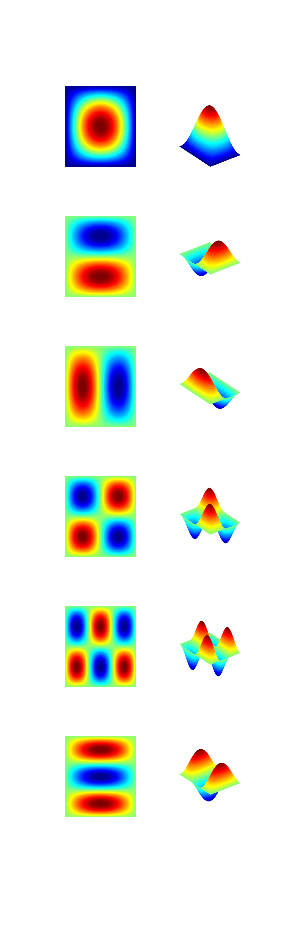
\includegraphics[width=\linewidth, height=18cm]{modes2.eps}
\end{center}
\caption{Modes pour une onde stationnaire en 2D. A gauche on peut voir une vue de haut et à droite une vue en 3D. De haut en bas , $m_{11}$,$m_{21}$,$m_{12}$,$m_{22}$,$m_{23}$,$m_{31}$}
\end{marginfigure}
Dans le cas d'une onde sonore et de conditions limites de déplacement nulles (il s'agit donc d'une boîte fermée), imposées sur toutes les faces d'un parallélépipède rectangle, l'équation d'onde pour $\xi$ devient: 
$$\xi(x,y,z,t)= A\sin(k_xx)\sin(k_yy)\sin(k_zz)\sin(\omega t)$$
Et les nombres d'ondes sont déterminés comme suit. Ils dépendent logiquement de leur longueur caractéristique respective.
$$ k_xL_x = m_x\pi \hspace{1cm} k_2y_y = m_y\pi \hspace{1cm} k_zL_z = m_z\pi$$
Il reste une chose à déterminer, la fréquence globale de l'onde. En insérant la solution trouvée dans l'équation d'ondes (\ref{eq:onde3D}), on obtient
$$ k = \sqrt{k_1^2+k_2^2+k_3^2} =\frac{2\pi}{\lambda}\hspace{3mm}\mbox{avec} \hspace{3mm} \omega = kv.$$ 

\section{Résonance}

D'une manière générale, on dit qu'il y a {\it résonance} lorsqu'un système réagit de façon beaucoup plus forte à des stimuli si ceux-ci sont à une (ou plusieurs) fréquence particulière. 

\noindent Les ondes stationnaires sont un cas typique de ce phénomène de résonance. Les modes propres d'un système peuvent facilement être activés par une petite sollicitation externe. L'exemple le plus courant est celui des instruments de musique pour lesquels une petite impulsion donne lieu à une réponse à une fréquence (ou un ensemble de fréquences) donnée: sur une corde vibrante dans le cas du piano, ou dans un tube pour le cas de la flûte. Les expériences menées au cours montrent aussi qu'une cavité de dimension bien choisie peut amplifier le son d'un diapason, et que celle-ci peut aussi se mettre à résonner sous l'impulsion des ondes sonores émises par un diapason voisin.


\noindent Il faut bien entendu noter que tous les phénomènes de résonance ne sont pas nécessairement liés à des ondes stationnaires. Il existe de multiples autres causes de résonance (circuits électriques, ressort, pendule, etc.)



\section{Battements}
Nous quittons ici le monde des ondes stationnaires pour étudier le phénomène de battement.
%Il s'agit de la variation de l'amplitude de la somme de plusieurs ondes.
Le phénomène est particulièrement reconnaissable lorsque deux ondes sonores de fréquence proche sont mélangées. Le résultat est que l'observateur perçoit une seule onde sonore à la fréquence moyenne, mais dont l'amplitude varie en fonction du temps à une vitesse qui dépend de la différence des deux fréquences. Ce phénomène n'est bien sur pas limité aux ondes sonores et s'applique à tous types d'ondes.

Calculons mathématiquement le résultat du mélange de deux ondes de fréquences proches mais différentes. Les deux ondes sont données par
$$ \xi_a=A_a\cos(\omega_at+\phi_a-\vec{k_a}\cdot\vec{r})$$
$$ \xi_b=A_b\cos(\omega_bt+\phi_b-\vec{k_b}\cdot\vec{r})$$
Pour simplifier les calculs, considérons que les ondes sont d'amplitudes identiques, de même polarisation, que leurs phases sont égales à $0$ et qu'elles se propagent toutes les deux à la même vitesse $v$ dans la direction de l'axe des $x$: $A_a=A_b=A$, $\phi_a=\phi_b=0$, $\vec{k_a}=\frac{\omega_a}{v}\hat{e_x}=k_a\hat{e_x}$ et $\vec{k_b}=\frac{\omega_b}{v}\hat{e_x}=k_b\hat{e_x}$. La somme des ondes peut s'écrire comme
$$ \xi=A\cos(\omega_at-k_ax) + A\cos(\omega_bt-k_bx)$$
$$ \xi=2A\cos\left(\frac{\omega_a+\omega_b}{2}t-\frac{k_a+k_b}{2}x\right)\cos\left(\frac{\omega_a-\omega_b}{2}t-\frac{k_a-k_b}{2}x\right).$$
Nous observons que le résultat est le produit de deux signaux: un premier signal dont la fréquence est la moyenne des deux fréquences sources; un second dont la fréquence est la moitié de la différence entre les deux fréquences sources. Le premier signal est celui que l'on entend, le deuxième est responsable de la variation d'amplitude. A noter que, assez logiquement, l'ensemble du signal se propage bien entendu toujours à la même vitesse $v$ dans la direction de l'axe des $x$. Le phénomène est représenté à la figure \ref{fig:battement}. On observe un signal à une fréquence proche de la fréquence des deux signaux, mais l'amplitude de ce signal dépend du temps. On peut le caractériser par son enveloppe, qui varie de façon sinusoïdale. La fréquence de cette enveloppe sinusoïdale est donnée par $$f_{env}=\frac{f_a-f_b}{2},$$ avec $\omega_a=2\pi f_a$ et $\omega_b=2\pi f_b$. 
Il faut néanmoins distinguer deux choses, la fréquence de l'enveloppe n'est pas celle que l'on entend comme variation d'amplitude. En effet pour notre oreille, même une valeur négative de l'enveloppe est entendue exactement comme une positive, il faut donc prendre la valeur absolue de l'enveloppe pour obtenir la fréquence de battement que l'oreille humain entend, et que l'on peut aussi caractériser par la fréquence des passages par zéro de l'amplitude:
$$f_{audible}=f_a-f_b.$$
\begin{marginfigure}[-10cm]\centering
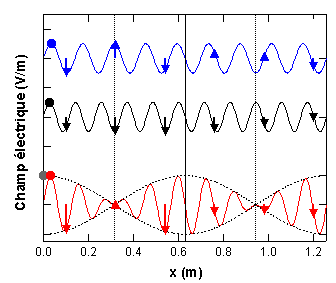
\includegraphics[width=\linewidth]{battement2}
\caption{Illustration du battement. Les deux ondes sources en bleu et noir. L'onde résultante en rouge. Nous pouvons observer la variation d'amplitude de l'onde résultante ainsi que son enveloppe.}
\label{fig:battement}
\end{marginfigure}
